
%%%%%%%%%%%%%%%%%%%%%%% file typeinst.tex %%%%%%%%%%%%%%%%%%%%%%%%%
%
% This is the LaTeX source for the instructions to authors using
% the LaTeX document class 'llncs.cls' for contributions to
% the Lecture Notes in Computer Sciences series.
% http://www.springer.com/lncs       Springer Heidelberg 2006/05/04
%
% It may be used as a template for your own input - copy it
% to a new file with a new name and use it as the basis
% for your article.
%
% NB: the document class 'llncs' has its own and detailed documentation, see
% ftp://ftp.springer.de/data/pubftp/pub/tex/latex/llncs/latex2e/llncsdoc.pdf
%
%%%%%%%%%%%%%%%%%%%%%%%%%%%%%%%%%%%%%%%%%%%%%%%%%%%%%%%%%%%%%%%%%%%


\documentclass[runningheads]{llncs}
\usepackage{amsmath}
\usepackage{mathtools}
\usepackage{amssymb}
\usepackage{float}
\usepackage{multicol}

\setcounter{tocdepth}{3}
\usepackage{graphicx}
\usepackage[sorting=none]{biblatex}
\addbibresource{references.bib}



\usepackage{url}
\urldef{\mailsc}\path||
\newcommand{\keywords}[1]{\par\addvspace\baselineskip
\noindent\keywordname\enspace\ignorespaces#1}

\begin{document}

\mainmatter  % start of an individual contribution

% first the title is needed
\title{Application of a chain-like and a hypercube communication topologies 
in a multi-swarm PSO algorithm applied to continuous optimization problems}
% Los titulos no llevan punto al final - M
% Maybe this is a bit too long? Also, it would be best to say *why*
% you did this, instead of what you did - JJ

% a short form should be given in case it is too long for the running head
\titlerunning{Appli. of comm. topologies in multi-swarm PSO}

% the name(s) of the author(s) follow(s) next
%
% NB: Chinese authors should write their first names(s) in front of
% their surnames. This ensures that the names appear correctly in
% the running heads and the author index.
%
\author{José Guzmán \and Mario García-Valdez \and Juan J. Merelo-Guervós}

\authorrunning{Guzmán et al.}
% (feature abused for this document to repeat the title also on left hand pages)

% the affiliations are given next; don't give your e-mail address
% unless you accept that it will be published
\institute{Tijuana Institute of Technology, Tijuana, Mexico
  \email{jose.guzmanc19@tectijuana.edu.mx, mario@tectijuana.edu.mx} \and
University of Granada, Spain, \email{jmerelo@ugr.es}}



%
% NB: a more complex sample for affiliations and the mapping to the
% corresponding authors can be found in the file "llncs.dem"
% (search for the string "\mainmatter" where a contribution starts).
% "llncs.dem" accompanies the document class "llncs.cls".
%

\toctitle{}
\tocauthor{José Guzmán, Mario García-Valdez}

\maketitle


\begin{abstract}

  Using multiple-swarm PSO is a technique used in recent years to help improve
  the performance of nature-inspired optimization algorithms. A distributed PSO
  algorithm can work in each swarm in parallel and also communicate particles
  between them asynchronously. However, the design of these systems is not a
  trivial task because many architectural options affect the exploration and
  exploitation of the search space. In this paper, we focus on proposing and
  comparing two communication policies regarding which swarms can communicate
  with each other. These policies intend to limit the communication between
  populations to increase exploration and avoid premature convergence. The
  proposed policies are chain and hypercubic topologies. We implemented them
  following an event-based cloud-native design. We compared the three options
  using several continuous optimization benchmark functions to assess the
  benefits of changing a communication topology. After the experiments, the
  chain topology had a better performance using MSE as a metric.
  
  
  % Probably rewrite it. Why did you do it? Why did
                  % you think it would work? - JJ
 % Done - Mario 
 % Edit at will - Mario
                   

\keywords{PSO, EvoSwarm, multi-swarm intelligence, communication topologies,
 chain algorithm, hypercube, multi-swarm PSO.}
\end{abstract}


\section{Introduction}

% 1. State the context
% 2. State the problem
% 3. Say the hypothesis you want to prove in the paper, its objective.
% 4. Say how you want to prove that hypothesis.

Among the various strategies that have emerged in recent times for bio-inspired
optimization algorithms, the creation of multiple populations working
in parallel and (possibly) asynchronously has proven to be valuable in 
solving complex optimization problems \cite{a1}.
Researchers often divide the original population into small sub-populations for some
purposes, for example, solving large-scale optimization problems and dynamic
optimization problems. Existing studies on multi-population optimization show
that it integrates easily into various nature-inspired optimization algorithms,
and often performs better than using single-population optimization algorithms
including global reference functions and real-world applications \cite{b11} \cite{b12}.
Other investigations, reviews, and surveys on multi-population methods have also
been published in recent years, in which multi-population concepts are described
using other terms like 'parallel,' 'Cooperative,' 'co-evolution,' and 'islands.'
Its multi-threaded and parallel processing features that significantly speed up
deployment time \cite{b13} \cite{b14}.

One of the critical points in this technique is communication between
populations, since it has been observed in various studies that the
exchange of possible solutions helps to improve the performance of
optimization algorithms \cite{a2}. The following four parameters
control communication between sub-populations:

\begin{itemize}
    \item A communication speed that defines the number of solutions in a sub-population to share with other sub-populations.
    \item A communication policy that determines which solutions should be replaced by those of other sub-populations.
    \item A communication interval that establishes the frequency to execute the communication.
    \item A connection topology that defines how to connect sub-populations.
\end{itemize}

Several distributed architectures have been proposed to manage the communication
and parallel execution of these kind of algorithms, for example there is a
similar approach by Scott Haberson et al. using a multi-population parallel
genetic algorithm for independent evolution \cite{da1}. 

In this paper, we propose the two communication topologies to be implemented in a 
even-based distributed multi-swarm Particle Swarm Optimization (PSO) algorithm.
These comminication topologies follow a chain and a hypercube structure on a milti-swarm. We chose
these topologies for their ability to be adapted to the architecture
mentioned above. They can work without altering the optimization
algorithm allowing a fair comparison with other communication
methods. 

This paper contains the following sections: We present state-of-the-art on
multi-swarm optimization in Section 2. In Section 3, we present the topologies,
and in Section 4, we present experimental setup and results, Furthermore,
Section 5 presents the conclusions for this work.

\section{State of the Art}

Particle Swarm Optimization (PSO) is an optimization algorithm
inspired flocks of birds or schools of fish. Since it was introduced in 1995 by  J. Kennedy and
R. Eberhar, it has undergone several improvements \cite{b1}. % pon el nombre del autor - M -j
Since then, researchers have created different versions, which aimed at different
purposes, developed new applications in many areas, published theoretical
studies on the effects of various parameters, and proposed many many
algorithm variants \cite{b2}. A basic version of the PSO algorithm
works with a population (swarm) of possible solutions
(particles). These particles move in the search space according to
some simple formulas. The movements in the particles' search space are
determined by their best known position and by the best known position
of the entire swarm. As better positions are discovered, they will
guide the swarm's movements. The process is repeated many times, so it
is expected that a satisfactory solution will eventually be
discovered, although this may not happen\cite{b3}.

Multi-swarm optimization is a variant of Particle Swarm Optimization
(PSO) based on multiple swarms (or sub-swarm) instead of one. The basic flow in
a multi-swarm optimization is that each sub-swarm focuses on a specific search
space region. In contrast, a specific diversification method decides where and
when to launch the sub-swarms.

For example, Wave of Swarm of Particles \cite{b6} bases its
diversification technique on the "collision" of particles. When the
particles are close to each other, they are sent into new sub-swarms,
preventing complete convergence. The Dynamic Multi-Swarm-Particle
Swarm Optimizer\cite{b7} regroups the particles from the sub-swarms
(if they have converged) into new sub-swarms periodically, so the new
iteration of swarms are started with particles from the previous
one. Locust swarms \cite{b8} are founded on a "devour and go" strategy
after a sub-swarm "devours" a small fraction of the search space. In
order to find a local optimum, explorers are deployed to search for
new regions promising to "keep going." 

In contrast to typical PSO swarms, sub-swarms are fed with information about
previous swarms. These could be the positions and velocities instead of having
their initial parameters to be randomly selected. In general, the development of
multi-swarm systems creates a new path of design decisions that did not exist
during the original development of PSO. These design decisions have been have
well-established guidelines thanks to the numerous studies on the topic, for
example, the use of non-random initial positions and initial velocities leads to
better re-sults in multi-swarm systems, which is not the case for individual
swarms \cite{b9}.

Some of these decisions can be reached by relatively independent
subcomponents that allow different optimization techniques to be
tested. For example, the multi-swarm system UMDA-PSO \cite{b10}
combines elements of particle swarm optimization, distribution
estimation algorithm, and differential evolution in a multi-swarm
hybrid method. % The whole introduction should go to State of the art
               % - JJ 
               % This is the SoA - M
There have been some papers focused in optimizing the communication
between swarms, for example the survey in reference \cite{b15} has a
collection of different investigations around this subject. For
example El-Abd and Kamel discussed the multiple factors that can
change the behavior of multiple cooperating swarms, these factors
included the communication strategy used and the number swarms. The
experimental results demonstrated that a circular topology
communication strategy has an overall better performance than those
that simple share the global best of all the swarms\cite{b16}. 

Another example and the source of inspiration for this paper, is one
of Li and Zeng, who presented a multi-population agent based
co-genetic algorithm with a chain-like structure for parallel global
numerical optimization, where a close chain-like connection structure,
a cycle chain-like connection structure and a dynamic neighborhood
were used to improve the parallel optimization\cite{b17}. 

In the next section, we present two variants of communication topologies,
to be used in an event-based architecture for the implementation of 
distributed population-based optimization algorithms.

\section{Proposed method}

Recently, there is an interest in cloud-native, event-based architectures
suitable to run locally on a personal computer or in a cloud platform service.
An event-based architecture uses events to trigger and communicate between
services and processes. Using an event-based architecture, we intend to carry
out a series of experiments to analyze the effect of changing the communication
topology in a multi-population optimization algorithm's performance. Using this
type of architecture with a multi-swarm optimization algorithm is a new
approach. Therefore, there is an opportunity to find a substantial variation in
the performance of such an optimization algorithm by changing the way the
various swarms communicate to exchange information.

First, we briefly present the overall architecture of EvoSwarm, the 
platform in which we implemented the distributed algorithm. 

EvoSwarm follows an event-based architecture, using message queues for
interprocess communication. Messages consist of small populations or swarms that
are consumed by worker processes that run a local PSO for a small number of
iterations. After this, the resulting swarm is pushed to another message queue
to be consumed by a migration process responsible for the communication
(migration) between swarm messages kept in a buffer \cite{b18}.
% Better a higher-level description, describing what's in
            % the queues. Also, message queues. - JJ

            % (See Figure \ref{fig:example}).

% \begin{figure}[h]
% \centering
% \DeclareGraphicsExtensions{.jpg}
% 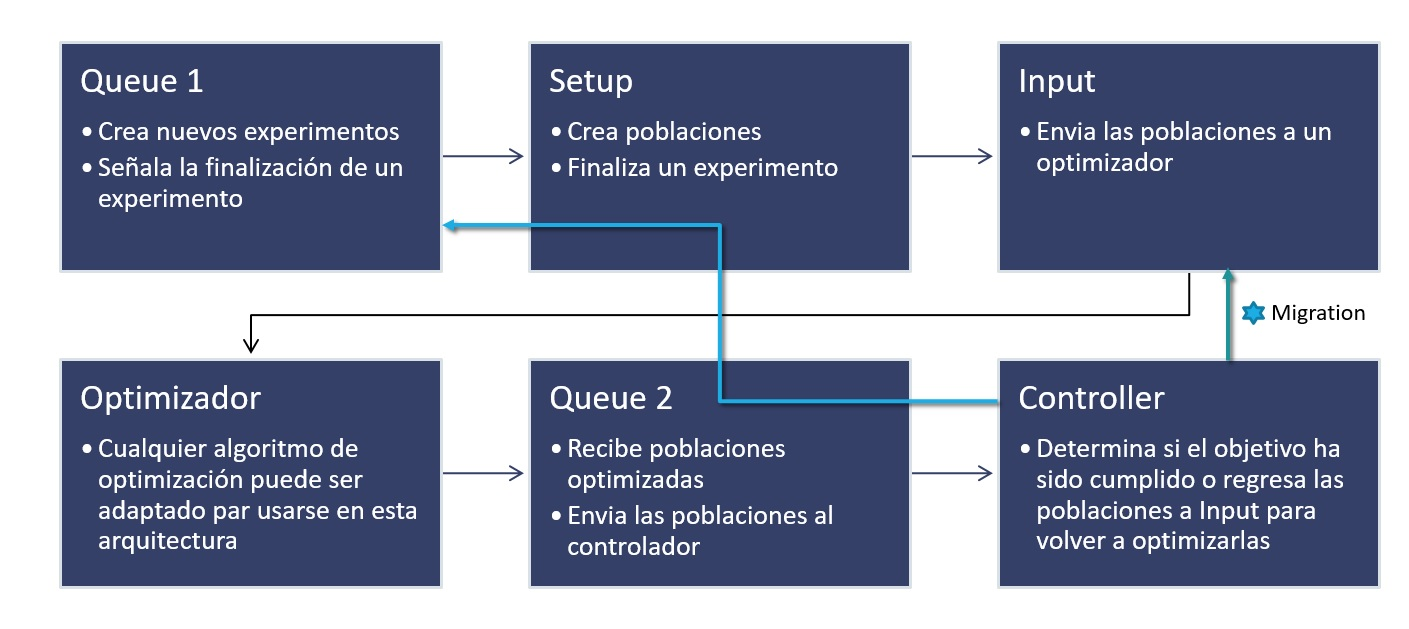
\includegraphics[scale=.40]{Resources/F1-1.jpg}
% \caption{The EvoSwarm flow.}
% \label{fig:example}
% \end{figure}
% Eliminated. It's in Spanish...

It is worth mentioning that this architecture can be implemented using various
computers in a network or using virtualization, in work we used Docker containers. 
Here are some of the most important features that
EvoSwarm brings to the user:

\begin{itemize} 
  
  \item Fully capable of scalability, since more computers can be added to the
  network in order to manage a more significant workload.
    
    \item Independence between processes, which means that any process in the
    structure is completely separated from the other ones allowing more work to
    be done at the same time.
    
    \item It is adaptable to any population-based optimizing algorithm.
\end{itemize}

The only change made to the original version of EvoSwarm \cite{b18} was the communication policy between the
populations of the multi-swarm PSO.

\subsection{PSO} 

%Aqui mover a como esta en tesis We implemented the software in

We implemented the migration policies in Python; for the PSO algorithm, we use the Evolopy library \cite{b19}, as mentioned
earlier in this paper, we use the same parameters for the PSO algorithm as the
EvoSwarm paper (see Table 1).

\begin{table}[h!]
\centering
\caption{Parameters PSO of Evolopy libray}
\begin{tabular}{|c c|} 
 \hline
 Parameters & Values  \\ [0.5ex] 
 \hline\hline
 Vmax & 6 \\ 
 Wmax & 0.9 \\
 Wmin & 0.2 \\
C1 & 2 \\
C2 & 2 \\[0.5ex]
 \hline
\end{tabular}
\label{table:1}
\end{table}

\subsection{EvoSwarm} 

Continuing with the configuration of the experiments, Table 2 presents the
parameters used in EvoSwarm; these are for the 3 cases presented in this paper.

\begin{table}[h]
\centering
\caption{Parameters for EvoSwarm}
\scalebox{0.90}{
\begin{tabular}{|c c c c c|} 
 \hline
 Dimensions & Generations  & Population size & Num. Experiments & Num. Population created\\ [0.2ex] 
 \hline\hline
 10 & 50 & 70 & 30 & 10 \\ 
 20 & 66 & 100 & 30 & 10 \\[0.2ex]
 \hline
\end{tabular}}
\label{table:1}
\end{table}

\subsection{Benchmark Functions}
%Aqui poner ref del pdf de coco

In order to run the optimization experiments, we selected ten functions from the
COCO benchmark. We selected these functions because in our preliminary
experiments, they showed performance variations as we changed the communication
topology. Here are the ten functions:

\begin{multicols}{2}
\begin{itemize}

    \item Function 1: Sphere.
    \item Function 2: Elipsoid separable.
    \item Function 3: Rastrigin separable.
    \item Function 9: Rosenbrock rota-ted.
    \item Functions 10: Elipsoid.
    \item Function 15: Rastrigin.
    \item Function 17: Schaffer F7, condition 10.
    \item Function 18: Schaffer F7, condition 1000.
    \item Function 21: Gallagher 101 peaks.
    \item Function 22: Gallagher 21 peaks

\end{itemize}
\end{multicols}

The number given to each function comes from COCO. This means that any method
using the benchmark can be compared against a great variety of optimization
methods. The complete collection of functions, graphics, and equations can be
reviewed in reference \cite{bbob}.

%\subsection{EvoSwarm communication topology} 
% These sections are too
% short and could be merged - JJ
%diagrama maybe % ok Mario

In the original communication policy, the architecture waited until a minimum of
three populations reached the migration component. These populations are sent to
a process that combines the best half of each one with the others. For example,
let us name the three populations A, B, and C, then a sort method is applied to
each one (based on the quality of the solution). The sorted populations are now
divided into halves in preparation for the merging process, now, with three new
populations, the first one has the best half of A and B, the second has the best
of B and C, and the third has the best of A and C. The last step is reinserting
these new populations into a queue from which the PSO processes will retake
them.

The first modification, in this case, is only on the merging process. To create
a chained algorithm that affects every three arriving populations, we sort the
three populations. The modification consists in that the populations are only
allowed to share a few members of the elite. In this case, 10. Individuals are
carried into a chain structure in which a population can receive only one way of
the structure and shares in another.

The 2nd variation for the EvoSwarm structure is a hypercube; we based this one
on a paper in which this topology was applied to solve a multi-reservoir of
water using a multi-population algorithm \cite{b20}. The name indicates this
method has a cubic structure and can only function with eight populations or
more. For this paper, we only need eight populations. Once the algorithm gets
filled with eight populations, the migrations algorithm needs to assign each one
a place in the hypercube structure. Figure 3 it has shown the layout of the
structure.

The structure resembles a cube, and in every one of its vertices is one
population. One thing that stands immediately is the capital P because only four
populations have it. In this algorithm, we divided the hypercube into two
dimensions. Moreover, depending on the iteration of the experiment, the exchange
of solutions is restricted.

Every iteration of an experiment changes the mode in which the populations
communicate with each other. For example, in the first iteration, the eight
populations can only communicate with the others in the same dimension. In the
second iteration, the opposite happens, allowing them to exchange information
with a population outside that dimension. With eight vertices, only two
exchanges are allowed, and for the experiments on this paper, only the best 10\%
of solutions migrate to another swarm.

\section{Experimental Results}

% Add some information about how the experiments were performed, type
% of machine, how much time they took ... -JJ
The experiments where made in a single computer using a Ryzen 5 2600x and 24 gb of ram, using the tecnology of docker 10 virtual computers were created for the process. Each experiment was conducted separetly and the standar time to do one, is about 6 to 8 hours.

Table 3 shows the different MSE obtained in the experimentation. % Also,
% you need to comment these results JJ

\begin{table}[h!tb]
    \centering
    \caption{Comparison of MSE obtained with the experiments, best results are in bold}
    \scalebox{0.72}{
    \begin{tabular}{|c|c||c|c|c||c|c|c|}
    \hline
     Dimensions & Function & EvoSwarm MSE & Chain MSE & Hypercube MSE & EvoSwarm Stdev & Chain Stdev & Hypercube Stdev \\ [0.5ex] 
    \hline\hline
    10 & 1	& \textbf{3.73447E-09} &	4.43163E-09 & 4.31567E-09 & 2.34E-09 & 2.68525E-09 & 3.10095E-09 \\ 
    10 & 2 & \textbf{3.78687E-09} & 4.88483E-09 & 3.95527E-09 & 2.84285E-09 & 2.46615E-09 & 2.95704E-09\\
    10 & 3 & 0.795723668 & \textbf{0.066330607} & 0.736180347 & 1.720290002 & 0.252429203 & 2.09770153 \\
    10 & 9 & 0.317521615 & \textbf{0.291698111} & 0.495606846 & 0.221999486 & 0.133724951 & 0.992888643 \\
    10 & 10 & 385.5382883 & \textbf{368.3836667} & 504.1392548 & 399.9278681 & 453.6655356 & 558.1741402 \\
    10 & 15 & 15.76249501 & \textbf{12.76554083} & 13.58271757 & 6.088547227 & 4.814606813 & 6.470316492 \\
    10 & 17 & \textbf{0.068348159} & 0.089892078 & 0.108848139 & 0.097958037 & 0.203665048 & 0.188877178 \\
    10 & 18 & 0.361780116 & \textbf{0.308286435} & 0.536340776 & 0.307789471 &0.364641853 & 0.53188395 \\
    10 & 21 & 0.241362711 & 0.330200323 & \textbf{0.129516888} & 0.518278881 & 0.588559758 & 0.343623139 \\
    10 & 22 & 0.58421438 & \textbf{0.337485965} & 0.947592035 & 0.698924145 & 0.614376298 & 1.092855278 \\
    20 & 1 & 5.5855E-09 & \textbf{5.29107E-09} & 5.60977E-09 & 2.54598E-09 & 3.08721E-09 & 2.78851E-09 \\
    20 & 2 & 0.70300253 & 2.214098553 & \textbf{5.51067E-09} & 3.850503404 & 12.12711719 & 2.43854E-09 \\
    20 & 3 & 8.506782382 & \textbf{6.523271752} & 6.566336254 & 7.91517587 & 6.962162793 & 6.445378042 \\
    20 & 9 & 11.75981164 & \textbf{11.28483752} & 11.54803115 & 1.257101321 & 1.070210208 & 1.150081504 \\
    20 & 10 & 5154.23155 & \textbf{4194.776213} & 4928.296717 & 4024.704045 & 3326.837717 & 4838.931553 \\
    20 & 15 & 57.76524461 & \textbf{55.55811032} & 58.12969092 & 16.78744293 & 17.2761844 & 13.78413645 \\
    20 & 17 & 0.807747361 & \textbf{0.65407833} & 0.87077806 & 0.377015722 & 0.323050832 & 0.450119262 \\
    20 & 18 & 2.648213694 & \textbf{2.136768786} & 2.51764207 & 1.402620032 & 0.898650887 & 1.195657371 \\
    20 & 21 & 0.624442455 & 0.2262255 & \textbf{0.2041556} & 0.903817073 & 0.486727692 & 0.513631785 \\
    20 & 22 & 2.030148903 & \textbf{1.578348414} & 1.915845972 & 1.821498605 & 1.638408845 & 1.869210661\\
    \hline
    \end{tabular}}
    \label{tab:my_label}
\end{table}
\hfill\break


%\subsection{Statistical test} % This should not be a different
                              % section. Statistical tests are always
                              % needed - JJ
We present the statistical tests below to compare the three methods
applied in this work, comparing the two new methods with the original
method and between them. In this case, we use a \(Z\) statistical test
with an $\alpha$ of 0.5, giving a critical value to exceed 1.64 that 
when surpassed signifies that the MSE in the right of the comparisson 
has sufficient evidence of having a minor MSE; % meaning? - JJ
in Table 4, the comparison between the EvoSwarm method and the Chain
method can be observed. Table 5 shows the comparison between EvoSwarm
and the Hypercube method. Finally, Table 6 is the comparison between
the methods and the Hypercube chain.\hfill \break
% You should simply show which comparisons are significant in the
% previous table - JJ
% Please add the following required packages to your document preamble:
% \usepackage{booktabs}
\begin{table}
\caption{Statistical comparison for EvoSwarm vs Chain method, positive test results are in bold}
    \scalebox{0.99}{
\begin{tabular}{|c|c|c|c|c|c|}
  \hline
  % If the z critic value is always the same, there's no need to
  % include it - JJ 
Dimension & Function & EvoSwarm MSE & Chain MSE  & EvoSwarm vs Chain Z value & Z critic value \\
\hline
10        & 1        & 4.7861E-09   & 4.4579E-09 & 0.38385888                    \\
10        & 2        & 3.8305E-09   & 4.1792E-09 & -0.51477671                   \\
10        & 3        & 2.35292757   & 0.53764944 & \textbf{3.04132131}           \\
10        & 9        & 0.49249742   & 0.2527938  & 1.31849085                    \\
10        & 10       & 250.173833   & 430.542073 & -1.71933543                   \\
10        & 15       & 14.6650026   & 12.0546942 & \textbf{1.64153098}           \\
10        & 17       & 0.0923583    & 0.07576297 & 0.3984427                     \\
10        & 18       & 0.52485291   & 0.50641272 & 0.12824242                    \\
10        & 21       & 0.32985228   & 0.23742293 & 0.64359863                    \\
10        & 22       & 0.69206415   & 0.51478211 & 1.05251019                    \\
20        & 1        & 0.03594249   & 5.5523E-09 & 0.99999998                    \\
20        & 2        & 5.6467E-09   & 5.4975E-09 & 0.23720531                    \\
20        & 3        & 12.082746    & 8.74663868 & 1.57882461                    \\
20        & 9        & 11.1034972   & 11.370252  & -0.5302659                    \\
20        & 10       & 4994.88899   & 4472.97104 & 0.55192392                    \\
20        & 15       & 58.8810247   & 53.5457402 & 1.09914007                    \\
20        & 17       & 0.78895834   & 0.76687862 & 0.19644001                    \\
20        & 18       & 2.53338619   & 2.25526688 & 1.10707452                    \\
20        & 21       & 0.90170655   & 0.39256696 & \textbf{2.09733952}           \\
20        & 22       & 3.6252321    & 1.51828786 & \textbf{2.6846472}            \\
\hline
\end{tabular}}
\end{table}
%EvoSwarm vs Hypercube
\begin{table}
\caption{Statistical comparison for EvoSwarm vs Hypercube method, positive test results are in bold}
    \scalebox{0.90}{
\begin{tabular}{|c|c|c|c|c|c|}
\hline
Dimension & Function & EvoSwarm MSE & Hypercube MSE  & EvoSwarm vs Hypercube Z value & Z critic value \\
\hline
10 & 1  & 4.78611E-09 & 4.52861E-09 & 0.30205024 \\
10 & 2  & 3.83054E-09 & 4.65155E-09 & -1.19206785 \\
10 & 3  & 2.352927573 & 0.805637277 & \textbf{2.54675887} \\
10 & 9  & 0.49249742  & 0.229809004 & 1.45323968   \\
10 & 10 & 250.1738327 & 374.4359744 & -1.71949324 \\
10 & 15 & 14.66500256 & 13.33777036 & 0.80707958   \\
10 & 17 & 0.0923583   & 0.087059177 & 0.12041284   \\
10 & 18 & 0.524852914 & 0.413659866 & 0.82306364  \\
10 & 21 & 0.329852279 & 0.20667313  & 0.91847447  \\
10 & 22 & 0.692064149 & 0.57179096  & 0.75725758   \\
20 & 1  & 0.03594249  & 5.54663E-09 & 0.99999998   \\
20 & 2  & 5.64673E-09 & 5.36566E-09 & 0.40712309  \\
20 & 3  & 12.082746   & 7.874205319 & \textbf{1.99114048}   \\
20 & 9  & 11.10349719 & 11.49485451 & -1.16267417 \\
20 & 10 & 4994.888993 & 5805.968994 & -0.60965616 \\
20 & 15 & 58.88102471 & 56.38870042 & 0.46747275  \\
20 & 17 & 0.788958338 & 0.764906251 & 0.20135086  \\
20 & 18 & 2.533386188 & 2.559019459 & -0.0776709  \\
20 & 21 & 0.901706552 & 0.395204608 & \textbf{2.23899811}   \\
20 & 22 & 3.625232097 & 1.650088133 & \textbf{2.59133147}  \\
  \hline
  % Best to present MSE +- StdDev, it's not so visual in different columns
\end{tabular}}
\end{table}

%Chain vs Hypercube

\begin{table}[h!tb]
\caption{Statistical comparison for Chain vs Hypercube method, positive test results are in bold}
    \scalebox{0.99}{
\begin{tabular}{|c|c|c|c|c|c|}
\hline
Dimension & Function & Chain MSE & Hypercube MSE  & Chain vs Hypercube Z value & Z critic value \\
\hline
10 & 1  & 4.4579E-09 & 4.5286E-09 & -0.08393014  \\
10 & 2  & 4.1792E-09 & 4.6515E-09 & -0.62905414  \\
10 & 3  & 0.53764944 & 0.80563728 & -0.64672855 \\
10 & 9  & 0.2527938  & 0.229809   & 0.66826276   \\
10 & 10 & 430.542073 & 374.435974 & 0.49686142   \\
10 & 15 & 12.0546942 & 13.3377704 & -0.88253544  \\
10 & 17 & 0.07576297 & 0.08705918 & -0.26448643  \\
10 & 18 & 0.50641272 & 0.41365987 & 0.84096876   \\
10 & 21 & 0.23742293 & 0.20667313 & 0.27151497   \\
10 & 22 & 0.51478211 & 0.57179096 & -0.3220766  \\
20 & 1  & 5.5523E-09 & 5.5466E-09 & 0.00809714  \\
20 & 2  & 5.4975E-09 & 5.3657E-09 & 0.18397258   \\
20 & 3  & 8.74663868 & 7.87420532 & 0.43285509   \\
20 & 9  & 11.370252  & 11.4948545 & -0.26587439  \\
20 & 10 & 4472.97104 & 5805.96899 & -1.20027498  \\
20 & 15 & 53.5457402 & 56.3887004 & -0.57885803  \\
20 & 17 & 0.76687862 & 0.76490625 & 0.01653624   \\
20 & 18 & 2.25526688 & 2.55901946 & -0.94401758  \\
20 & 21 & 0.39256696 & 0.39520461 & -0.01355104  \\
20 & 22 & 1.51828786 & 1.65008813 & -0.34473831  \\
\hline
\end{tabular}}
\end{table}
\hfill
\break

% There does not seem to be a big difference, and none at all between
% the different technologies. You should comment on this, and why it
% happens on these specific functions - JJ

\section{Conclusions}

In this research, we compared three communication methods between
populations of a multi-swarm system to identify the variation in the
result caused by these changes. However, the difference between most
of the results is not very large.
% Discussion should include why this happens, and why there are
% differences in specific circumstances or functions. Also if there's
% some change with the problem size (dimensions) - JJ

Nevertheless, there are scenarios in
which the change was quite relevant, so it is possible to say that the
change in communication policies significantly impacts multi-swarm
methods for continuous optimization. In the same way, we must take
into account that in this case, we only changed the type of
communication between sub-swarms, which is only one of the policies
that we can alter in this type of system. In future works, other
policies can be altered at the same time to see what impact they will
have. With the results obtained, we can infer that the change to the
communication method is relevant for this type of system in specific
situations. The alteration of the different work policies in
multi-swarm systems could lead to greater specialization of these in
specific scenarios.

\section*{Acknowledgments}

This paper has been supported in part by project DeepBio (TIN2017-85727-C4-2-P).


\printbibliography


\end{document}
